%%%%%%%%%%%%%%%%%%%%%%%%%%%%%%%%%%%%%%%%%
% a0poster Portrait Poster
% LaTeX Template
% Version 1.0 (22/06/13)
%
% The a0poster class was created by:
% Gerlinde Kettl and Matthias Weiser (tex@kettl.de)
%
% This template has been downloaded from:
% http://www.LaTeXTemplates.com
%
% modifications: cyrillic letters in Rnw + xetex
% https://github.com/bdemeshev/templates/tree/master/poster_rnw_xtex
% 12.01.2016
%
% License:
% CC BY-NC-SA 3.0 (http://creativecommons.org/licenses/by-nc-sa/3.0/)
%
%%%%%%%%%%%%%%%%%%%%%%%%%%%%%%%%%%%%%%%%%



%----------------------------------------------------------------------------------------
%	PACKAGES AND OTHER DOCUMENT CONFIGURATIONS
%----------------------------------------------------------------------------------------

\documentclass[a0, landscape]{a0poster}

% by default knitr uses 'color' package
% we replace it by 'xcolor':


%\usepackage[T1]{fontenc}
%\usepackage[utf8]{inputenc}
%\usepackage[british, russian]{babel}
%\usepackage{type1ec} %

%\usepackage{fontspec}
%\usepackage{polyglossia}

% \setmainlanguage{russian}
% \setotherlanguages{english}

% download "Linux Libertine" fonts:
% http://www.linuxlibertine.org/index.php?id=91&L=1
% \setmainfont{Times New Roman} % or Helvetica, Arial, Cambria
% why do we need \newfontfamily:
% http://tex.stackexchange.com/questions/91507/
% \newfontfamily{\cyrillicfonttt}{Times New Roman}

\usepackage{mathtext}          % русские буквы в формулах

\usepackage[utf8]{inputenc}         % кодировка исходного текста
\usepackage[british]{babel} % локализация и переносы



\usepackage{multicol} % This is so we can have multiple columns of text side-by-side
\columnsep = 100pt % This is the amount of white space between the columns in the poster
\columnseprule = 3pt % This is the thickness of the black line between the columns in the poster

\usepackage[svgnames]{xcolor} % Specify colors by their 'svgnames', for a full list of all colors available see here: http://www.latextemplates.com/svgnames-colors

%\usepackage{times} % Use the times font
%\usepackage{palatino} % Uncomment to use the Palatino font

\usepackage{graphicx} % Required for including images
\graphicspath{{figures/}} % Location of the graphics files
\usepackage{booktabs} % Top and bottom rules for table
\usepackage[font = small, labelfont = bf]{caption} % Required for specifying captions to tables and figures
\usepackage{amsfonts, amsmath, amsthm, amssymb} % For math fonts, symbols and environments
\usepackage{wrapfig} % Allows wrapping text around tables and figures
\newcommand{\cIW}{\mathcal{IW}}
\newcommand{\prior}{\underline}
\newcommand{\cN}{\mathcal{N}}

\begin{document}

%----------------------------------------------------------------------------------------
%	POSTER HEADER
%----------------------------------------------------------------------------------------

% The header is divided into two boxes:
% The first is 75% wide and houses the title, subtitle, names, university/organization and contact information
% The second is 25% wide and houses a logo for your university/organization or a photo of you
% The widths of these boxes can be easily edited to accommodate your content as you see fit

\begin{minipage}[b]{0.75\linewidth}
\veryHuge \color{NavyBlue} \textbf{Forecasting of Russian Macroeconomic Indicators with BVAR} \color{Black}\\ % Title
%\Huge\textit{An Exploration of Complexity}\\[2cm] % Subtitle

\huge \textbf{Oxana Malakhovskaya$^{1,2}$, Boris Demeshev$^{1}$}\\[0.5cm] % Author(s)
\Large $^{1}$ Higher School of Economics\\[0.4cm] % University/organization
\Large $^{2}$ University of Paris-Saclay\\[0.4cm] % University/organization
\Large \texttt{omalakhovskaya@hse.ru, boris.demeshev@gmail.com} \\
\end{minipage}
%
\begin{minipage}[b]{0.25\linewidth}
%
\includegraphics[width=10cm]{hse_logo.png}
%\includegraphics[width=15cm]{logo_ps.png}

\includegraphics[width=20cm]{both_logos.png}
\end{minipage}

\vspace{1cm} % A bit of extra whitespace between the header and poster content

%----------------------------------------------------------------------------------------

\begin{multicols}{3} % This is how many columns your poster will be broken into, a portrait poster is generally split into 2 columns


\large


%----------------------------------------------------------------------------------------
%	ABSTRACT
%----------------------------------------------------------------------------------------

%\color{Navy} % Navy color for the abstract
%
%\begin{abstract}
%
%\Large
%
%This paper evaluates the forecast performance of Bayesian vector autoregressions (BVARs) on Russian data. We estimate BVARs of different sizes and compare the accuracy of their out-of-sample forecasts with those obtained with unrestricted vector autoregressions and random walk with drift. We show that many Russian macroeconomic indicators can be forecast by BVARs more accurately than by competing models. However, contrary to several other studies, we do not confirm that the relative forecast error monotonically decreases with increasing the cross-sectional dimension of the sample. In half of those cases where a BVAR appears to be the most accurate model, a small-dimensional BVAR outperforms its high-dimensional counterpart.
%
%\end{abstract}

%----------------------------------------------------------------------------------------
%	INTRODUCTION
%----------------------------------------------------------------------------------------

\color{SaddleBrown} % SaddleBrown color for the introduction

% \section*{Introduction}
%
%
%
%
% \textit{Aliquam auctor}, metus id ultrices porta, risus enim cursus sapien, quis iaculis sapien tortor sed odio. Mauris ante orci, euismod vitae tincidunt eu, porta ut neque. Aenean sapien est, viverra vel lacinia nec, venenatis eu nulla. Maecenas ut nunc nibh, et tempus libero. Aenean vitae risus ante. Pellentesque condimentum dui. Etiam sagittis purus non tellus tempor volutpat. Donec et dui non massa tristique adipiscing.

%----------------------------------------------------------------------------------------
%	OBJECTIVES
%----------------------------------------------------------------------------------------

\color{Black} % DarkSlateGray color for the rest of the content

\section*{Motivation}
\begin{itemize}
\item Recently many papers has claimed that, in terms of forecasting accuracy, medium and large BVAR outperform their small dimensional counterparts.
\item Application of Bayesian econometrics on Russian data is scarce
\end{itemize}

\section*{Main Objectives}

\begin{itemize}
\item Forecasting of macroeconomic indicators for Russian economy with BVARs of different size
\item Comparing their forecasting accuracy with one of competing models (RW and unrestricted VARs)
\end{itemize}

\section*{Main Hypotheses}

\begin{itemize}
\item BVARs outperform the competing models in terms of forecasting accuracy
\item High-dimensional BVARs forecast better than low-dimensional ones
\end{itemize}

\section*{Model}
The model written in a compact way:
\begin{equation*}
Y=X\Phi+E,\label{var}
\end{equation*}

where $Y=[y_1, y_2,\ldots, y_T]'$,$X=[x_1, x_2,\ldots, x_T]'$, $x_t=[ y'_{t-1} \ldots  y'_{t-p} \; 1]'$,  $\Phi=[\Phi_1 \ldots \Phi_p \; \Phi_{c}]'$, $E=[\varepsilon_1, \varepsilon_2,\ldots, \varepsilon_T]'$ with\\

\begin{itemize}
\item  conjugate normal -- inverted Wishart prior
%
%
%
%%\section*{Prior distribution}
%
%The conjugate normal -- inverted Wishart prior:
%\begin{equation}
%\begin{cases}
%\Sigma\sim \cIW(\prior S, \prior \nu) \\
%\Phi | \Sigma \sim \cN (\prior\Phi, \Sigma \otimes \prior\Omega)
%\end{cases},
%\end{equation}
%%where $\prior \phi = \vec{ \prior \Phi}$ and:
%plus  two modifications:
%\begin{itemize}
\item sum-of-coefficients prior
\item initial observation prior
\end{itemize}
The overall tightness parameter is chosen endogenously depending on the sample dimension following (Banbura et al., 2010).

\section*{Our dataset}
\begin{itemize}
\item 23 monthly time series running from January 1996 to April 2015
\item Series demonstrating seasonal fluctuations are seasonally adjusted
\item Logarithms are applied to most of the series, with the exception of those already expressed in rates.
\end{itemize}


\subsection*{Estimated models}

\begin{center}
\begin{tabular}{ll}
\toprule
VAR3/BVAR3 & $Y=\lbrace IP, CPI, R \rbrace$\\
VAR4/BVAR4 & $Y=\lbrace IP, CPI, R, Z\rbrace$ \\
VAR6/BVAR6 & $Y=\lbrace IP, CPI, R, M2, REER, OPI \rbrace$ \\
VAR7/BVAR7 & $Y=\lbrace IP, CPI, R, M2, REER, OPI, W \rbrace$\\
BVAR23     & $Y$ includes all 23 variables from the dataset\\
\bottomrule
\end{tabular}
\end{center}
$IP$ - industrial product index, $CPI$ - consumer price index, $R$ - nominal interbank rate, $M2$ - monetary aggregate M2, $REER$ - real effective exchange rate, $OPI$ - Brent oil price index. $Z$ is any variable from the dataset besides $IP$, $CPI$ and $R$.  $W$ is any variable from the dataset besides $IP$, $CPI$, $R$, $M2$,$REER$, and $OPI$.

\subsection*{Estimation scheme}
\begin{center}
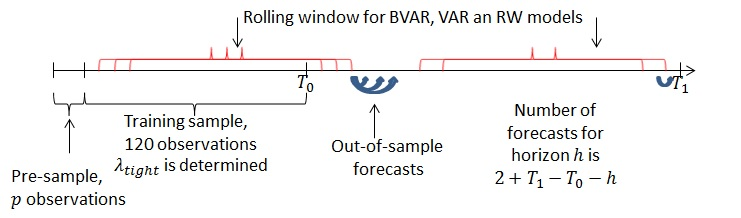
\includegraphics[scale=1.5]{estimation_scheme2}
\end{center}
%
%\subsection*{Forecast accuracy}
%
%Our indicator or  forecast accuracy is:
%\begin{equation}
%MSFE_{var,h}^{\lambda,m}=\frac{1}{T_1-T_0-h+1}\sum_{\tau=T_0}^{T_1-h} (y_{var,\tau+h|\tau}^{\lambda,m}-y_{var,\tau+h|\tau})^2
%\end{equation}
%
%We report relative MSFE:
%
%\begin{equation}
%RMSFE=\frac{MSFE_{var,h}^{\lambda,m}}{MSFE_{var,h}^0}
%\end{equation}
%where $var$ is any variable in the dataset, $MSFE_{var,h}^0$ is a MSFE of RW with drift.

%
\subsection*{Results}
In tables,  relative MSFE are reported.

\begin{equation*}
RMSFE=\frac{MSFE_{var,h}^{\lambda,m}}{MSFE_{var,h}^0}
\end{equation*}
\begin{center}
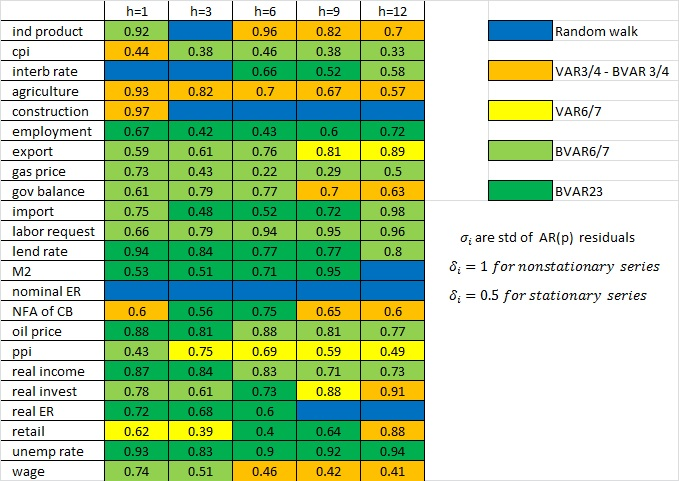
\includegraphics[scale=1.5]{hyper3}
\end{center}
\begin{center}
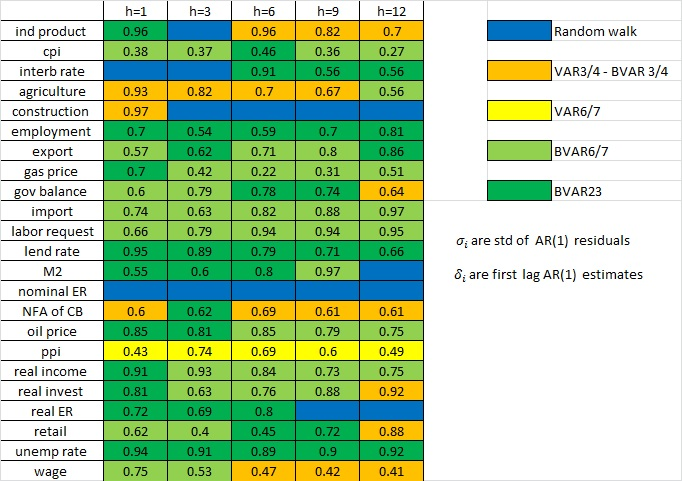
\includegraphics[scale=1.5]{hyper4}
\end{center}



\subsection*{Robustness check}
\begin{center}
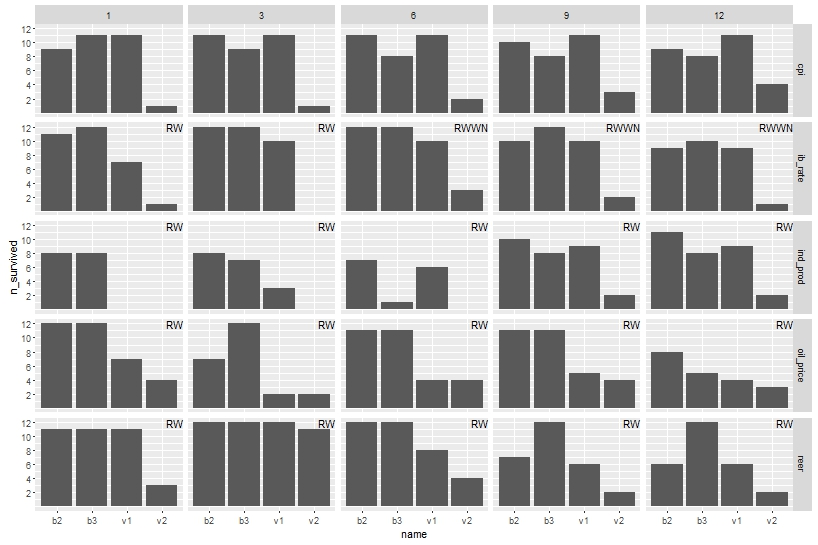
\includegraphics[scale=1]{model_selection}
\end{center}

%
%\subsection*{Interpretation of the results}
%\begin{itemize}
%\item For many variables and forecasting horizons in interest, BVAR outperforms random walk and unrestricted VAR.
%\item Though medium BVAR is the best option for some cases, it is often beaten by a BVAR model with relatively low number of variables (6 or 7).
%\item For some variables and some forecasting horizons VARs (either restricted or not) cannot beat RW, for example, nominal exchange rate (long-lasting consensus in economics)
%\item Nonetheless, the oil price index can be forecast by BVAR much better than by RW.
%\end{itemize}

\subsection*{Conclusion}
\begin{itemize}
\item In the paper, we estimate BVAR models of different size and compare their forecasting performance with RW with drift and unrestricted VAR models for 23 variables and 5 different forecast horizons.
\item We show that for a majority of variables of interest BVAR produces better forecasting results than the competing models.
\item However, we cannot confirm a conclusion of some studies that high-dimensional BVARs forecast better than low-dimensional models. For many variables in our sample and forecasting horizons a 6- or 7-variable BVAR can beat a 23-variable BVAR in terms of forecasting accuracy.
\end{itemize}



%%----------------------------------------------------------------------------------------
%%	MATERIALS AND METHODS
%%----------------------------------------------------------------------------------------
%---------------------------------------------------------------------------
%
%\section*{Results}
%
%Donec faucibus purus at tortor egestas eu fermentum dolor facilisis. Maecenas tempor dui eu neque fringilla rutrum. Mauris \emph{lobortis} nisl accumsan. Aenean vitae risus ante.
%%
%\begin{wraptable}{l}{12cm} % Left or right alignment is specified in the first bracket, the width of the table is in the second
%\begin{tabular}{l l l}
%\toprule
%\textbf{Treatments} & \textbf{Response 1} & \textbf{Response 2}\\
%\midrule
%Treatment 1 & 0.0003262 & 0.562 \\
%Treatment 2 & 0.0015681 & 0.910 \\
%Treatment 3 & 0.0009271 & 0.296 \\
%\bottomrule
%\end{tabular}
%\captionof{table}{\color{Green} Table caption}
%\end{wraptable}
%%
%Phasellus imperdiet, tortor vitae congue bibendum, felis enim sagittis lorem, et volutpat ante orci sagittis mi. Morbi rutrum laoreet semper. Morbi accumsan enim nec
%
%
%
%
%
%\begin{center}\vspace{1cm}
%
\includegraphics[width=0.8\linewidth]{placeholder}
%\captionof{figure}{\color{Green} Figure caption}
%\end{center}\vspace{1cm}
%
%In hac habitasse platea dictumst. Etiam placerat, risus ac.
%
%Adipiscing lectus in magna blandit:
%
%\begin{center}\vspace{1cm}
%\begin{tabular}{l l l l}
%\toprule
%\textbf{Treatments} & \textbf{Response 1} & \textbf{Response 2} \\
%\midrule
%Treatment 1 & 0.0003262 & 0.562 \\
%Treatment 2 & 0.0015681 & 0.910 \\
%Treatment 3 & 0.0009271 & 0.296 \\
%\bottomrule
%\end{tabular}
%\captionof{table}{\color{Green} Table caption}
%\end{center}\vspace{1cm}
%
%Vivamus sed nibh ac metus tristique tristique a vitae ante. Sed lobortis mi ut arcu fringilla et adipiscing ligula rutrum. Aenean turpis velit, placerat eget tincidunt nec, ornare in nisl. In placerat.
%
%\begin{center}\vspace{1cm}
%
\includegraphics[width=0.8\linewidth]{placeholder}
%\captionof{figure}{\color{Green} Figure caption}
%\end{center}\vspace{1cm}
%
%%----------------------------------------------------------------------------------------
%%	CONCLUSIONS
%%----------------------------------------------------------------------------------------
%
%\color{SaddleBrown} % SaddleBrown color for the conclusions to make them stand out
%
%\section*{Conclusions}
%
%
%\color{DarkSlateGray} % Set the color back to DarkSlateGray for the rest of the content
%
%%----------------------------------------------------------------------------------------
%%	FORTHCOMING RESEARCH
%%----------------------------------------------------------------------------------------
%
%\section*{Forthcoming Research}
%
%

 %----------------------------------------------------------------------------------------
%	REFERENCES
%----------------------------------------------------------------------------------------

%\nocite{*} % Print all references regardless of whether they were cited in the poster or not
%\bibliographystyle{plain} % Plain referencing style
%\bibliography{sample} % Use the example bibliography file sample.bib



\end{multicols}
\end{document}
